\chapter{Project Design}

\section*{Introduction}
After having specified the project requirements in the previous chapter, we introduce in this chapter,
the design of the "Pulpetech-Insights" project. In addition, we present the global architecture of the project.
Finally, we  zoom into the main layers of the project architecture and explain by providing accurate diagrams that describe it best.

\pagebreak

\section{Software Architecture Design}
\subsection{MVC design pattern}
Design patterns are a collection of modifications which may improve certain quality attributes.
Design patterns do not change the functionality of the system, only the organization or structure of that functionality.
Applying a design pattern generally affects only a limited number of classes in the architecture.
The quintessential example used to illustrate design patterns is the Model View Controller
(MVC) design pattern.

The MVC pattern, was originally developed by Professor Trygve Reenskaug at Xerox PARC in 1978.
This pattern \cite{mvc} is a way of breaking an application, or even just a piece of an application’s interface, into three parts: the model, the view, and the controller.
\begin{itemize}
    \item Model:
    Represents the business layer of the application.
    \item View:
    Defines the presentation of the application.
    \item Controller:
    Manages the flow of the application.
\end{itemize}

\begin{figure}[htbp!]
  \center
  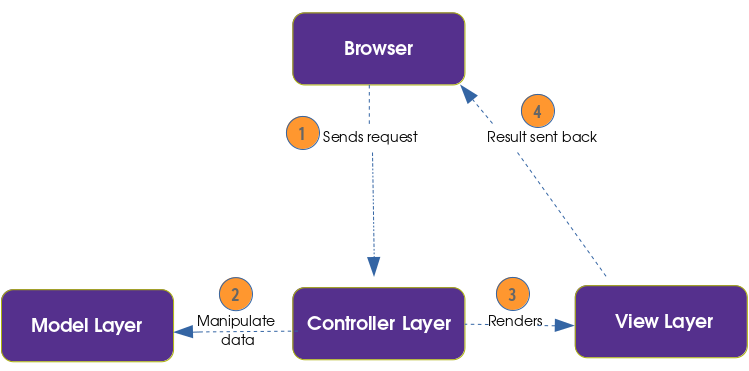
\includegraphics[width=16cm]{mvc_fig}
  \caption{MVC Architecture design}
  \label{fig:mvc_fig}
\end{figure}
The figure above \hyperref[fig:mvc_fig]{\ref{fig:mvc_fig}}  illustrates the MVC architecture interactions.

The use of this design pattern leads to greater flexibility and modifiability.
There is a clearly defined separation between components of program problems in each domain can be solved independently.
New views and controllers can be easily added without affecting the rest of the application.

%\vspace{100mm}

\subsection{Three-Tier Client Server Architecture}
A 3-tier application architecture is a modular client-server architecture that consists of a presentation tier, an application tier and a data tier. As the following figure \hyperref[fig:three]{\ref{fig:three}}  shows, the data tier stores information, the application (Business Logic) tier handles logic and the presentation tier is a graphical user interface (GUI) that communicates with the other two tiers. The three tiers are logical, not physical, and may or may not run on the same physical server.\cite{three}
\begin{figure}[h]
  \center
  \includegraphics[width=16cm]{three}
  \caption{Three-Tier Client Server Architecture}
  \label{fig:three}
\end{figure}

\subsection{REST architecture}
Rest stands for Representational State Transfer. It is an architecture style for designing
networked applications. It permits creating, modifying resources easily. Indeed REST is a
lightweight alternative to complex mechanism like RPC, CORBA and SOAP.

Rest is not a ’standard’. In fact, it is a guideline to build an efficient framework for
communication between two machines using HTTP protocol. The World Wide Web itself,
based on HTTP, can be viewed as a REST-based architecture. REST relies on a stateless,
client-server, cacheable communication protocol. It is simple to implement and maintain.
In addition, it allows applications to be scalable by supporting multiple backend services
at the same time.

Much like Web Services, a REST service is platform-independent, language-independent
standard-based as it runs on top of HTTP, and is easily used in the presence of firewalls.

However, there are a few major concepts which make REST unique from other web
services. In fact , its main key principals are the following:

$\bullet$ \textbf{Unique URL-Resource mapping}: Every resouce is mapped to a unique URL.
That refers to a some logical way to access information

$\bullet$ \textbf{Statelessness}: All information required to process the request by server is contained along with the request. This means that no information of the previous request is
maintained by the server. This is inherited from the fact that REST is based on HTTP.

$\bullet$ \textbf{Action Verbs}: REST architecture use HTTP verbs to identify the appropriate
action. The main HTTP verbs used in a REST architecture are GET, POST, PUT and
DELETE. In fact, GET is used by the client to access the resource on the server, PUT to
update a resource, POST to create a new one and DELETE to remove resource.

$\bullet$ \textbf{Data Exchange formats}: REST architecture does not require any particular
encoding for the resource body. JSON \cite{json} and XML are the most used format, but it can
be PROTOBUF, YAML etc.

The Pulpetech-Insights System will be developed under two main architectural styles/ patterns. 
Development of the project will be done in MVC architectural style and also 3 tier Client/Server Architecture.

\section{Static software architecture}
In this section, we will present the static software architecture of Pulpetech-Insights project.
\subsection{Diagram Class}
The class diagram is the heart of UML. It is based on the principles of object-orientation (abstraction, encapsulation, heredity, etc.) and due to its versatility can be implemented in all phases of a project. In the analysis phase, it appears as the domain model and attempts to provide an image of reality. The software is modeled with it in the design phase, and in the implementation phase source code is generated.
\begin{figure}[!htbp]
\center
\hspace*{-0.5in}
\includegraphics[width=18cm,height=14.2cm]{class-diagram}
  \caption{Pulpetech-Insights diagram class}
  \label{fig:diagram_class}
\end{figure}

%\subsection{Entity Relationship Diagram}
%An Entity Relationship Diagram (ERD) is a snapshot of data structures. An Entity Relationship Diagram shows entities (tables) in a database and relationships between tables within that database.
%The following figure  \hyperref[fig:erd]{\ref{fig:erd}} represents the entity relationship diagram of the project.
%
%
%\begin{figure}[h]
%\center
%\hspace*{-0.5in}
%\includegraphics[width=18cm,height=14cm]{erd}
%  \caption{Pulpetech-Insights ER diagram }
%  \label{fig:erd}
%\end{figure}
%
\subsection{Web services list}

The following table  \hyperref[fig:apis]{\ref{fig:apis}} represents the APIs used list on the project.

\begin{table*}[!htbp]

  \small
  \begin{center}
      \begin{tabular}{|p{0.1\textwidth}|p{0.3\textwidth}|p{0.2\textwidth}|p{0.4\textwidth}|}
      \toprule

      {\bf API group} & {\bf Methods \& URL} & {\bf Parameters} & {\bf Output}  
\\
      \midrule\midrule[.1em]
      \multirow{2}{1cm}{ML APIs} 
                      & GET  \hspace{5mm}{\tt /classify/polarity/}
                                   & {\tt review}%, {\tt tableWidth}%, {\tt schema} (optional)  
                                   & a review polarity \{Pos, Neg\}
                                   \\
      \cmidrule(lr){2-4}
                       & GET  \hspace{10mm} {\tt /classify/type/}
                                   & {\tt review}
                                   & a review Topic \{Shipping, Site, Product\} \\ 
  \midrule[.1em] 

      \multirow{2}{3.5cm}{User APIs} 
                                   & POST \hspace{20mm} {\tt /api/login/}
                                   & {\tt username}, {\tt password }
                                  & an access and refresh JSON web \\
      \cmidrule(lr){2-4}
                       & POST \hspace{20mm}  {\tt /api/reviews}
                      & {\tt username}
                                                      & a list of reviews \\   
  \cmidrule(lr){2-4}
                      &POST \hspace{10mm} {\tt /api/reviews/add}
                      & {\tt username}, {\tt review(s)}
                      & a result of adding process {success, failure}\\   

  \cmidrule(lr){2-4}
                      & POST \hspace{2mm}{\tt /api/reviews/status}
                                   & {\tt username},
                                   {\tt    status}
                                                      & the count of status reviews \\   

  \cmidrule(lr){2-4}
                                                      & POST {\tt /api/reviews/top\_word}
                         & {\tt username},
                         {\tt status}
                                    & a list of top used status words \\   

  \cmidrule(lr){2-4}
                      & POST \hspace{20mm}{\tt /api/reviews/type}
                                   & {\tt username}
                                                      & a filtred list of reviews\\   

  \cmidrule(lr){2-4}
                      & POST \hspace{2mm}{\tt /api/token/refresh/}
                                   & {\tt refresh JSON web token}
                                   & a status of the token\\   

  \cmidrule(lr){2-4}
                      & POST \hspace{30mm}{\tt /api/user}
                                   & {\tt username}
                                                      & the details of user\\   

  \cmidrule(lr){2-4}
                      &POST \hspace{15mm} {\tt /api/user/reviews}
                                   & {\tt username}
                                                      &  a list of reviews related of user\\   



  \cmidrule(lr){2-4}
                      & POST,GET,PUT,PATCH {\tt /users/}

                      & {\tt username}
                      {\tt email},%, first\_name, last\_name,password,logo \_url
                      {\tt first\_name},
                      {\tt last\_name},
                      {\tt password},
                      {\tt logo\_url}
                      &   a result of managing user process
                      \\   


      \midrule[.1em] 
    \end{tabular}
  \end{center}
    \caption{Pulpetech-Insights APIs}
    \label{fig:apis}

\end{table*}



\section{Dynamic software architecture}
UML Sequence Diagrams are interaction diagrams that detail how operations are carried out. They capture the interaction between objects in the context of a collaboration. Sequence Diagrams are time focus and they show the order of the interaction visually by using the vertical axis of the diagram to represent time what messages are sent and when.

$\bullet$ \textbf{Authentication sequence diagram :}
The below figure  \hyperref[fig:login_seq]{\ref{fig:login_seq}} illustrates the sequence diagram of the authentication use case.


\begin{figure}[!htbp]
\center
\hspace*{-0.5in}
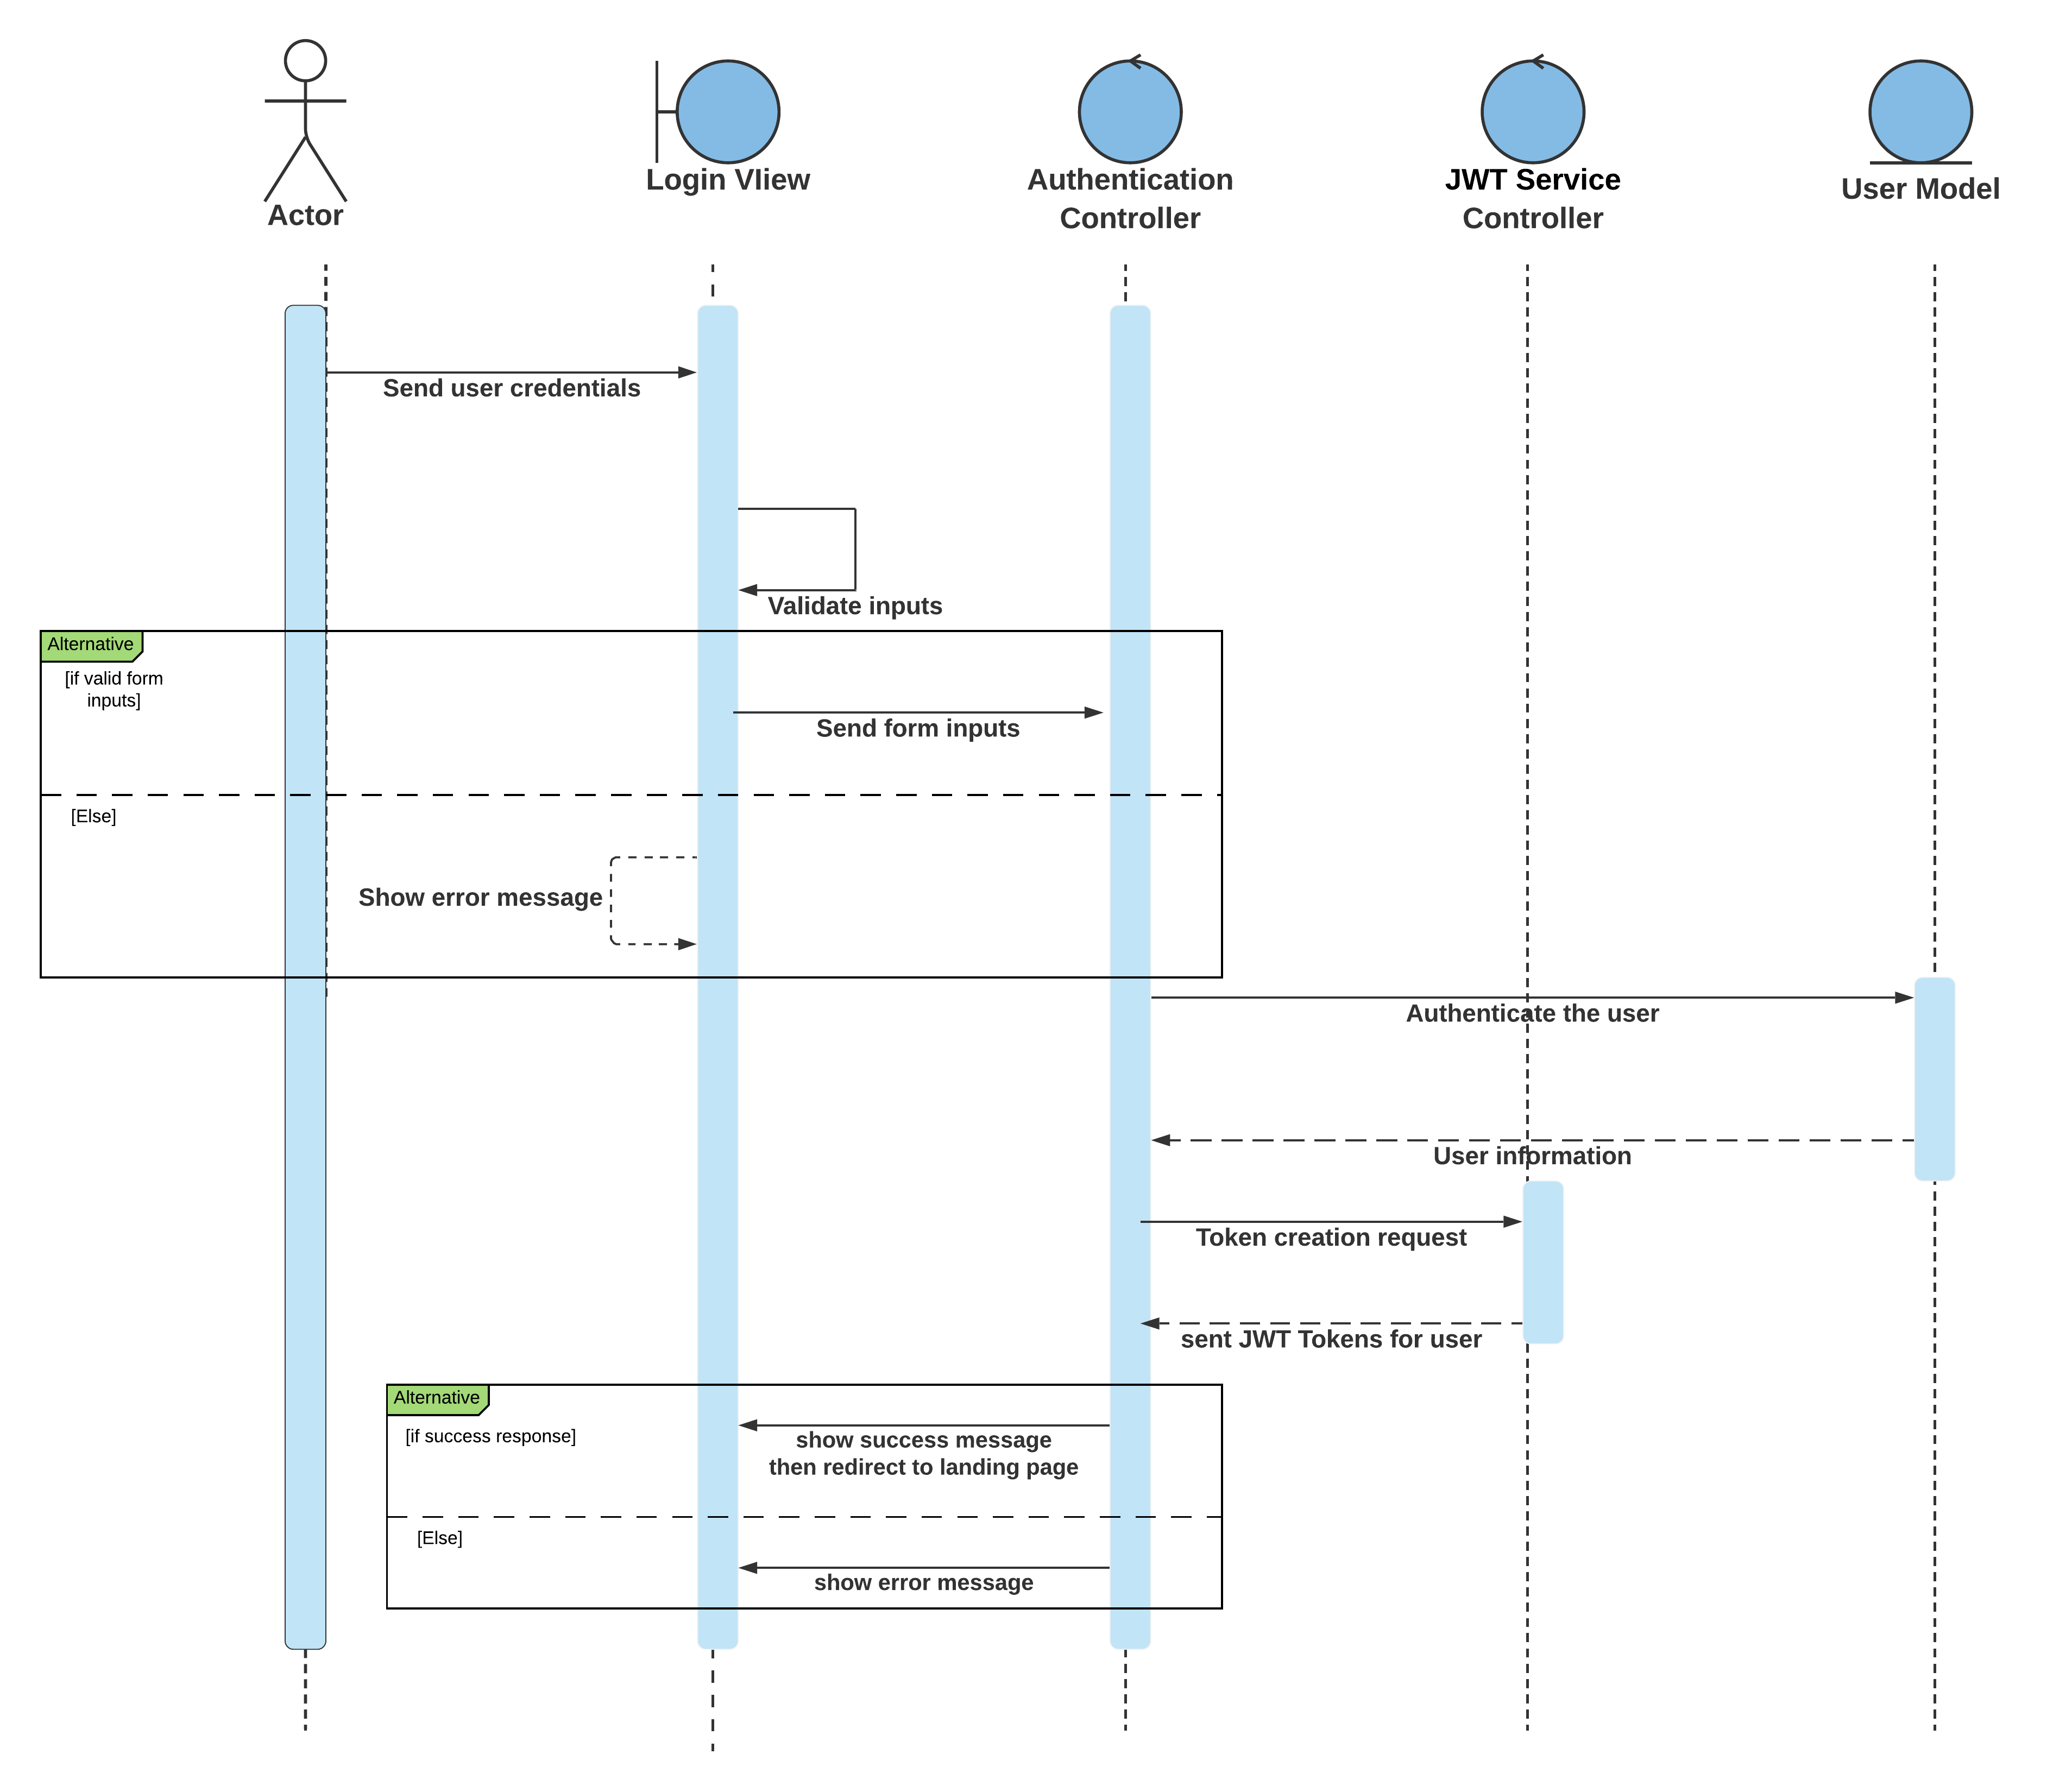
\includegraphics[width=18cm,height=14.6cm]{login_seq2}
  \caption{Authentication sequence diagram}
  \label{fig:login_seq}
\end{figure}


$\bullet$ \textbf{Upload data sequence diagram}: 

The below figure  \hyperref[fig:u_seq]{\ref{fig:u_seq}} illustrates the sequence diagram of upload data use case.


\begin{figure}[!htbp]
\center
\hspace*{-0.5in}
\includegraphics[width=18cm,height=17cm]{Update Sequence diagram}
  \caption{Upload data sequence diagram}
  \label{fig:u_seq}
\end{figure}

\section*{Conclusion}
In this chapter, we have defined software architecture design. 
This has led us to clearly identify the static software architecture that should achieve.
Presented system's web services then the dynamic software architecture by providing accurate diagrams that describe it thoroughly.
